\subsection{Domain Name System}

\emph{Domain Name System} (DNS) provides the mapping from the
human-readable name to IP address. A user asks DNS something
like "what is the IP address of www.google.com?" and DNS
responds "8.8.8.8".

The DNS infrastructure consists of local DNS servers
subordinate to centralized DNS servers managed by ICANN.

DNS has a hierarchical infrastructure. For example,
\texttt{ece.purdue.edu} (the ECE's domain) is a
subdomain of \texttt{purdue.edu} (Purdue's domain),
which is itself a subdomain of \texttt{edu} (the top level
domain for American educational institutions). Thus,
DNS infrastructure reflects this hierarchy. \texttt{ece.purdue.edu}
has a DNS server, \texttt{purdue.edu} has a DNS server,
and \texttt{edu} belongs to the set of generic domain servers.
The general hierarchy is:
\begin{enumerate}
    \item Root server: address hardwired into other DNS servers. Managed by ICANN/IANA
    \item Top Level Domain (TLD) servers: \texttt{.com}, \texttt{.uk} etc. Managed by ICANN/IANA
    \item Local DNS servers: \texttt{.purdue.edu}, \texttt{.google.com}. Managed by local service providers
\end{enumerate}

Every DNS server knows the address of the root server. Every DNS server
knows the address of its immediate children. A DNS server only stores the
name-to-address mappings of the domain it has authority for.
The DNS hierarchy is designed this way so that each server only
needs to store a subset of the DNS database, ensuring scalability, and
so that any server can discover servers for any portion of the hierarchy.

Each DNS server is typically replicated for availability and scalability.
The DNS service is available if there is at least one replica up.
Queries can be load balanced among replicas using \emph{anycast}.

A comparison of anycast and other destination IP addressing methods
follows:
\begin{itemize}
    \item unicast: one destination host
    \item broadcast: desintation is all hosts in the network
    \item multicast: subset of hosts in the network
    \item anycast: a group of receivers are associated with the
          same destination IP. A routing algorithm sends to a single
          receiver from the group based on some metric (e.g. least
          loaded receiver, geographically closest). Typically used to
          balance the load across multiple servers each running the
          same service
\end{itemize}

Say you, an entrepreneur, wants to start a university named
"The People's Northeastern University of Singapore".
You want to register the domain "pnus.com". The first step
is to get a block of IP addresses from your ISP, such as
\texttt{112.110.117.128/25}. Next, you register "pnus.com"
with a registrar like GoDaddy, which you provide with the
name and IP of your local DNS server(s). The registrar
will insert what you provide into the \texttt{.com} TLD
server. For instance, you might provide your registrar with
\texttt{dns1.pnus.com}, \texttt{112.110.117.115}. You
then store mappings for your domain in your local DNS server
\texttt{dns1.pnus.com}, such as
\begin{itemize}
    \item \texttt{www.pnus.com}: \texttt{112.110.117.110}
    \item \texttt{mail.pnus.com}: \texttt{112.110.117.100}
    \item \texttt{math.pnus.com}: \texttt{112.110.117.0}
\end{itemize}

Hosts on a network have a DNS client which triggers the resolver
code via, for instance, the command \texttt{gethostbyname()},
which then sends the DNS query to the local DNS server. If the
DNS doesn't have the associated IP, it may contact other DNS
servers to resolve the query before sending back the response
to the client.

In the DNS protocol there are \emph{query} and \emph{reply}
messages, which are carried over unreliable transport
such as UDP port 53. The DNS specification supports reliable
transport (TCP) too, but this is not always implemented.
Reliability is typically implemented via repeating requests
on timeout.

There are two ways to resolve a DNS query, as illustrated
by Figures \ref{fig:recursivedns} and \ref{fig:iterativedns}.

\begin{figure}
    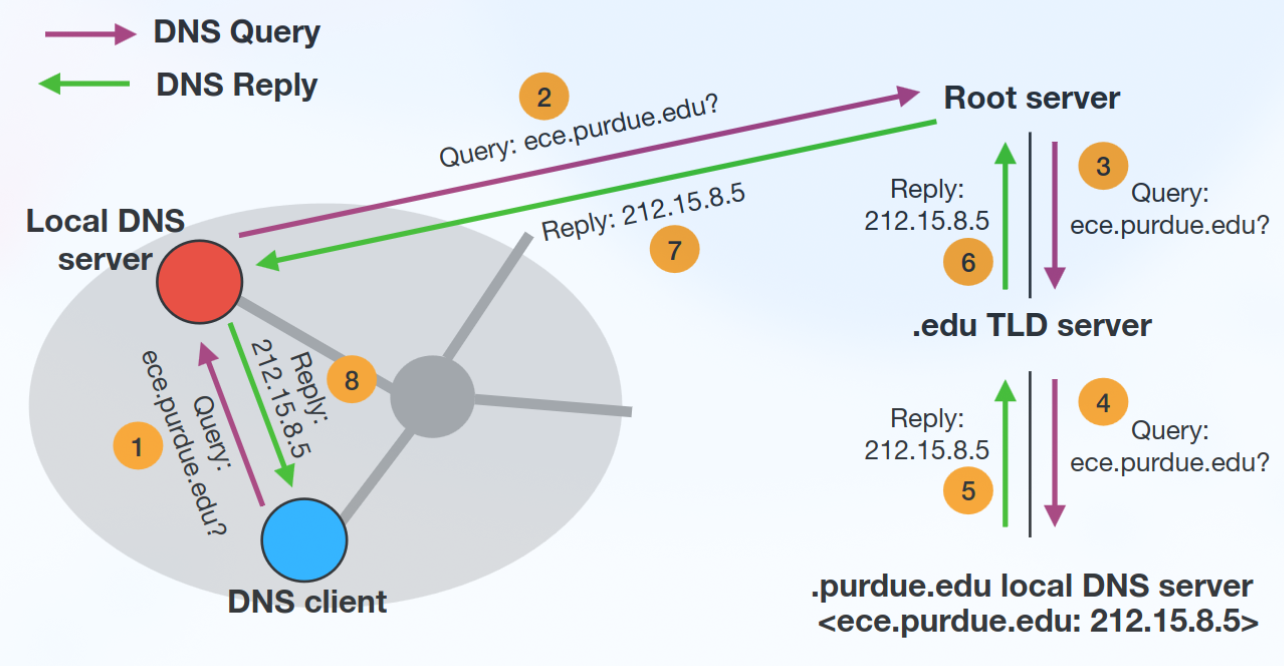
\includegraphics{images/recursivedns.png}
    \caption{Recursive DNS query resolution}
    \label{fig:recursivedns}
\end{figure}

\begin{figure}
    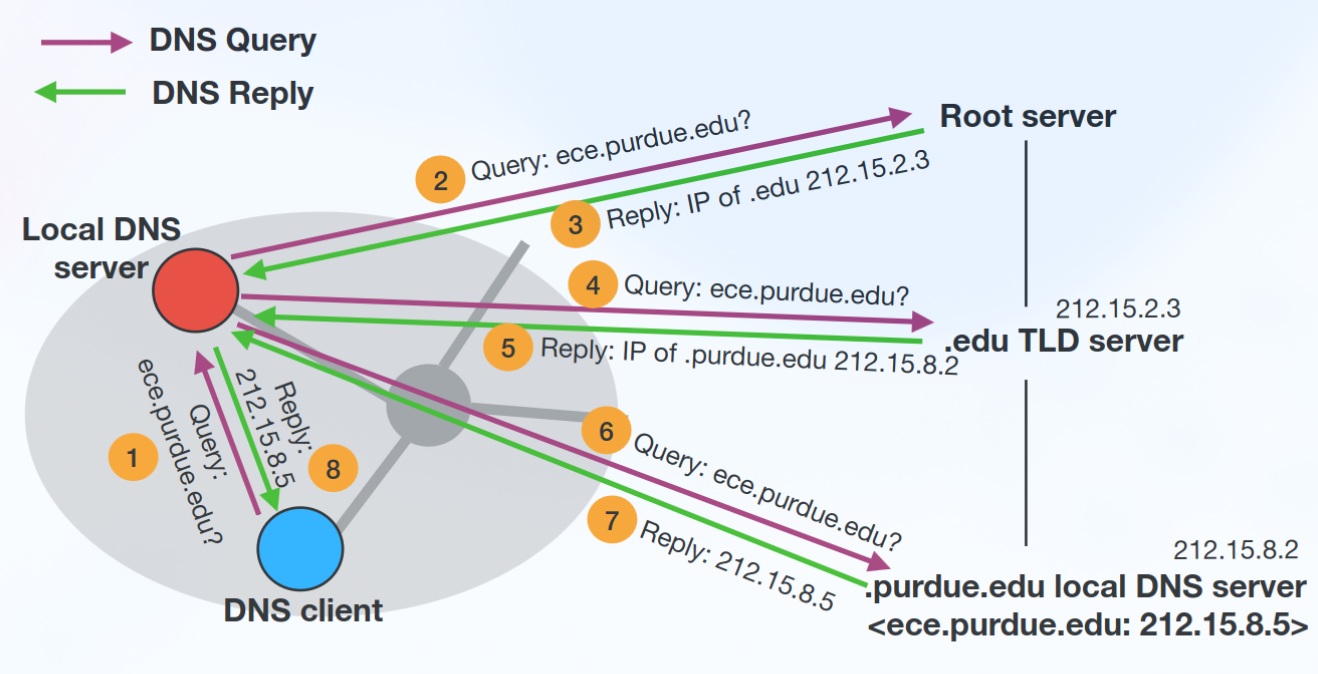
\includegraphics{images/iterativedns.png}
    \caption{Recursive DNS query resolution}
    \label{fig:iterativedns}
\end{figure}

All DNS servers at every level of the hierarchy reply to
queries. DNS replies include a \emph{time to live} (TTL)
field. The DNS server delete cached entries after the TTL
expires. Most popular queries hit the cache in the local
DNS server, which enables a faster reply to clients. DNS
caching can be done at the host for even faster reply.
Windows implements this by default, and applications such
as browsers can also implement their own DNS caching.